\section{Pitch rate command system}

Reducing the state space model in Equation~\ref{eq:sslon} by eliminating the velocity and pitch angle states result in the following model.

\begin{equation}
    \begin{aligned}
        A_{red}&=\begin{bmatrix}
            -0.05167 &   0.9792 \\
            -0.6256  & -0.2485
        \end{bmatrix} &
        B_{red}&=\begin{bmatrix}
            -0.0002308 \\
            -0.01541
        \end{bmatrix} \\\\
        C_{red}&=I_2 &
        D_{red}&=0_{2,1}
    \end{aligned}
\end{equation}

Simulating the step response for both models yields similar results. It is clear in the response of the full model that the short period is the dominant eigenmotion during the first few seconds. Since only the initial response of the system in relevant for the CAP and Gibson dropback criterion, it is fine to continue using the reduced model for the rest of the assignment.

\begin{figure}[ht]
    \centering
    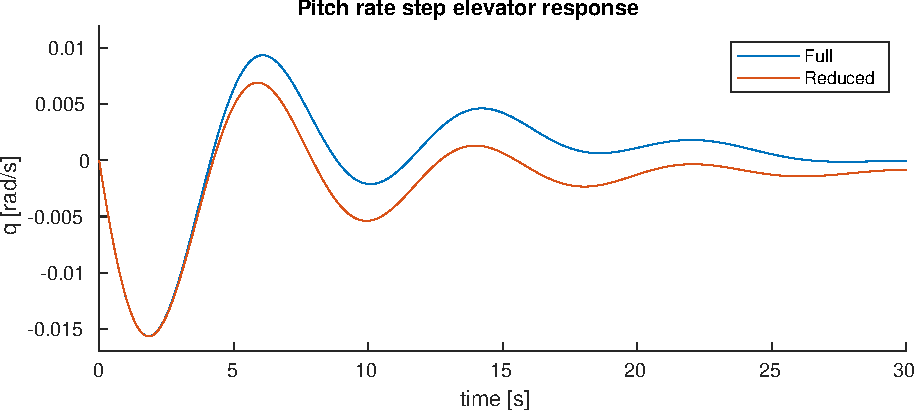
\includegraphics[width=0.6\textwidth]{figures/pc_acre_step.pdf}    
    \caption{Pitch rate elevator step response for both the full and reduced model.}
    \label{fig:pc_acre_step}
\end{figure}

A feedback loop is needed in order to satisfy the short period natural frequency and damping requirements. Figure~\ref{fig:pc_loop1} shows the control loop for solving this problem. The system $G$ is the open loop state space system and $K$ is the to be determined gain matrix.

\begin{figure}[ht]
    \centering
    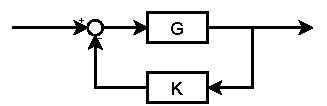
\includegraphics[width=0.4\textwidth]{figures/pc_loop1.pdf}    
    \caption{Feedback loop with gain in the loop.}
    \label{fig:pc_loop1}
\end{figure}

The build-in matlab function \texttt{place(...)} is used to calculate the gain $K_{reduced}$ using pole placement. The resulting gain is shown in Equation~\ref{eq:gaink}.

\begin{equation}
    \label{eq:gaink}
    K_{reduced}=\begin{bmatrix}
                    K_{\alpha} & K_q
                \end{bmatrix}
               =\begin{bmatrix}
                    -449.0440 & -151.8325
                \end{bmatrix}
\end{equation}

The new closed loop system matrix $A$ can then be calculated using Equation~\ref{eq:aclosed} and the rest of the matrices are the same as that of the open loop system. The new closed loop system can be found in Equation~\ref{eq:closedloopsystem}.

\begin{equation}
    \label{eq:aclosed}
    A_{closed} = A_{open}-B_{open}K
\end{equation}


\begin{equation}
    \label{eq:closedloopsystem}
    \begin{aligned}
        A_{closed}&=\begin{bmatrix}
            -0.1553 &  0.9442 \\
            -7.544  & -2.588 \\
        \end{bmatrix} &
        B_{closed}&=\begin{bmatrix}
            -0.0002308 \\
            -0.01541
        \end{bmatrix} \\\\
        C_{closed}&=I_2 &
        D_{closed}&=0_{2,1}
    \end{aligned}
\end{equation}

                                                                       
                                                                 

Calculating the damping and natural frequency of the closed loop system shows that the parameters match the required $\zeta=0.5$ and $\omega_n=0.03V\approx 2.74$
\begin{table}[h!]
    \centering
    \begin{tabular}{ c c c c c }
         Poles         & $\zeta$        & $\omega_n$ \\ \hline \hline
         $1.37 + 1.37i$ & $\e{5.00}{-1}$ & $2.74$     \\  
         $1.37 - 1.37i$ & $\e{5.00}{-1}$ & $2.74$     \\ \hline
    \end{tabular}
    \caption{Longitudinal eigenmotions poles, damping rations, natural frequencies, periods and time to half amplitude.}
\end{table}

If small angle approximations are assumed it is possible to calculate the angle of attack using the following equation.

\begin{equation}
    \alpha = \frac{w}{V}
\end{equation}

Here is $w$ the vertical airspeed component and V the total airspeed. Thus the angle of attack change in case of a vertical gust may be calculated by dividing the gust speed by the free stream velocity. This angle of attack may be passed as an initial condition to a simulation in order to observe the aircraft's behavior during such a gust. For a severe gust with $w=4.572\ [m\ s^{-1}]$ the initial angle of attack in the assigned flight condition is,

\begin{equation}
    \alpha_0=\frac{4.572\ [m\ s^{-1}]}{300\ [ft\ s^{-1}]}=\frac{4.572\ [m\ s^{-1}]}{91.44\ [m\ s^{-1}]} = 0.05\ [rad]
\end{equation}

The simulation results for both the open and closed loop systems using this initial condition and zero inputs is shown in Figure~\ref{fig:pc_vertgust}. As it can be seen the closed loop system quickly dampens the disturbance due the vertical gust, in contrast to the open loop system which continues oscillating significantly longer.

\begin{figure}[ht]
    \centering
    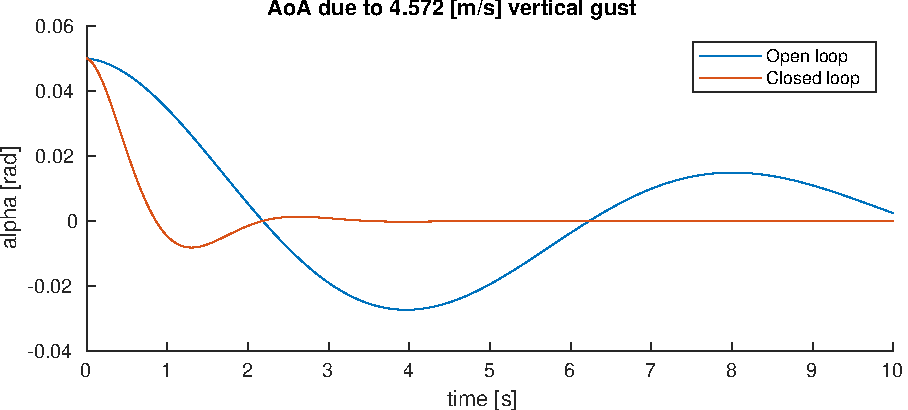
\includegraphics[width=0.6\textwidth]{figures/pc_vertgust.pdf}    
    \caption{Angle of attack during a $w=4.572\ [m\ s^{-1}]$ vertical gust for the open and closed loop systems.}
    \label{fig:pc_vertgust}
\end{figure}

The $T_{\theta_2}$ time constant cannot be modified by pole placement or by some other control loop structure. The reason is because it is located in the numerator of the transfer function and it's not possible to change the numerator using a feedback loop gain. 

Placing the lead-lag filter inside of the loop on the forward path will make it end up in both the numerator and denominator of the closed loop transfer function. Thus making it impossible to replace the zero without without changing the damping ratio and natural frequency of the closed loop system.

To modify $T_{\theta_2}$ a lead-lag prefilter can be placed before the closed loop system. The pole in the prefilter is used to cancel the current zero with $T_{\theta_2}$ in the closed loop, and the prefilter's zero end up in the overall transfer function, thus replacing the original zero.

\begin{equation}
    \frac{q(s)}{\delta_{el}(s)}=\frac{1+T_{\theta_2,new}}{1+T_{\theta_2,old}} \cdot
        \frac{k_q \left(1+T_{\theta_2,old}\right)}{
        s^2+2\zeta\omega_ns+\omega_n^2}
        =
        \frac{k_q \left(1+T_{\theta_2,new}\right)}{
        s^2+2\zeta\omega_ns+\omega_n^2}
\end{equation}

Even with the prefilter the controller will still not track the reference pitch rate signal properly, there will be a steady state error that needs to be compensated for. The reason is because the signal coming from the feedback loop is scaled by the gain $K$ and thus the reference signal needs to be scaled as well.

For this assignment the \texttt{rscale(...)} function which can be found at \cite{matlabrscale} is used. The final form of the precompensator is thus,

\begin{equation}
    N \cdot \frac{1+T_{\theta_2,new}}{1+T_{\theta_2,old}}
\end{equation}

Where $N$ is the scaling factor from \texttt{rscale(...)}.


% Category B: Those nonterminal Flight Phases that are normally accomplished using
% gradual maneuvers and without precision tracking, although accurate
% flight-path control may be required. Included in this Category are:

Figure~\ref{fig:pc_cap} shows the level 1 Control Anticipation Parameter criteria for Category B flight phases. According to \cite{milstd1797a}, Category B flights phases are normally accomplished using gradual maneuvers and without precision tracking, which includes cruise flight. As it can be seen, the controller satisfies the requirement.

\begin{equation}
    CAP=\frac{g\omega^2T_{\theta_2}}{V} \approx 0.1168
\end{equation}

\begin{figure}[ht]
    \centering
    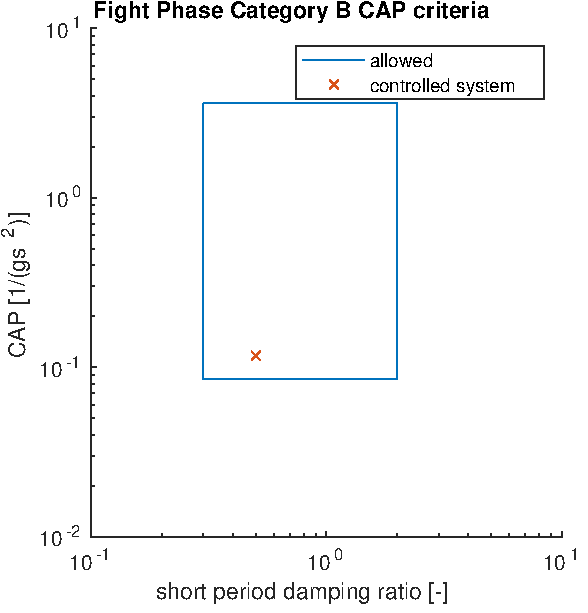
\includegraphics[width=0.4\textwidth]{figures/pc_cap.pdf}    
    \caption{Control Anticipation Parameter criteria for Category B flight phases and the location for the controlled system in the plot.}
    \label{fig:pc_cap}
\end{figure}

Figure~\ref{fig:pc_cap} shows the pitch rate and pitch angle step response of the controlled system. The maximum pitch rate $q_m$ and steady state value $q_s$ are marked in the plot. 
\begin{figure}[ht]
    \centering
    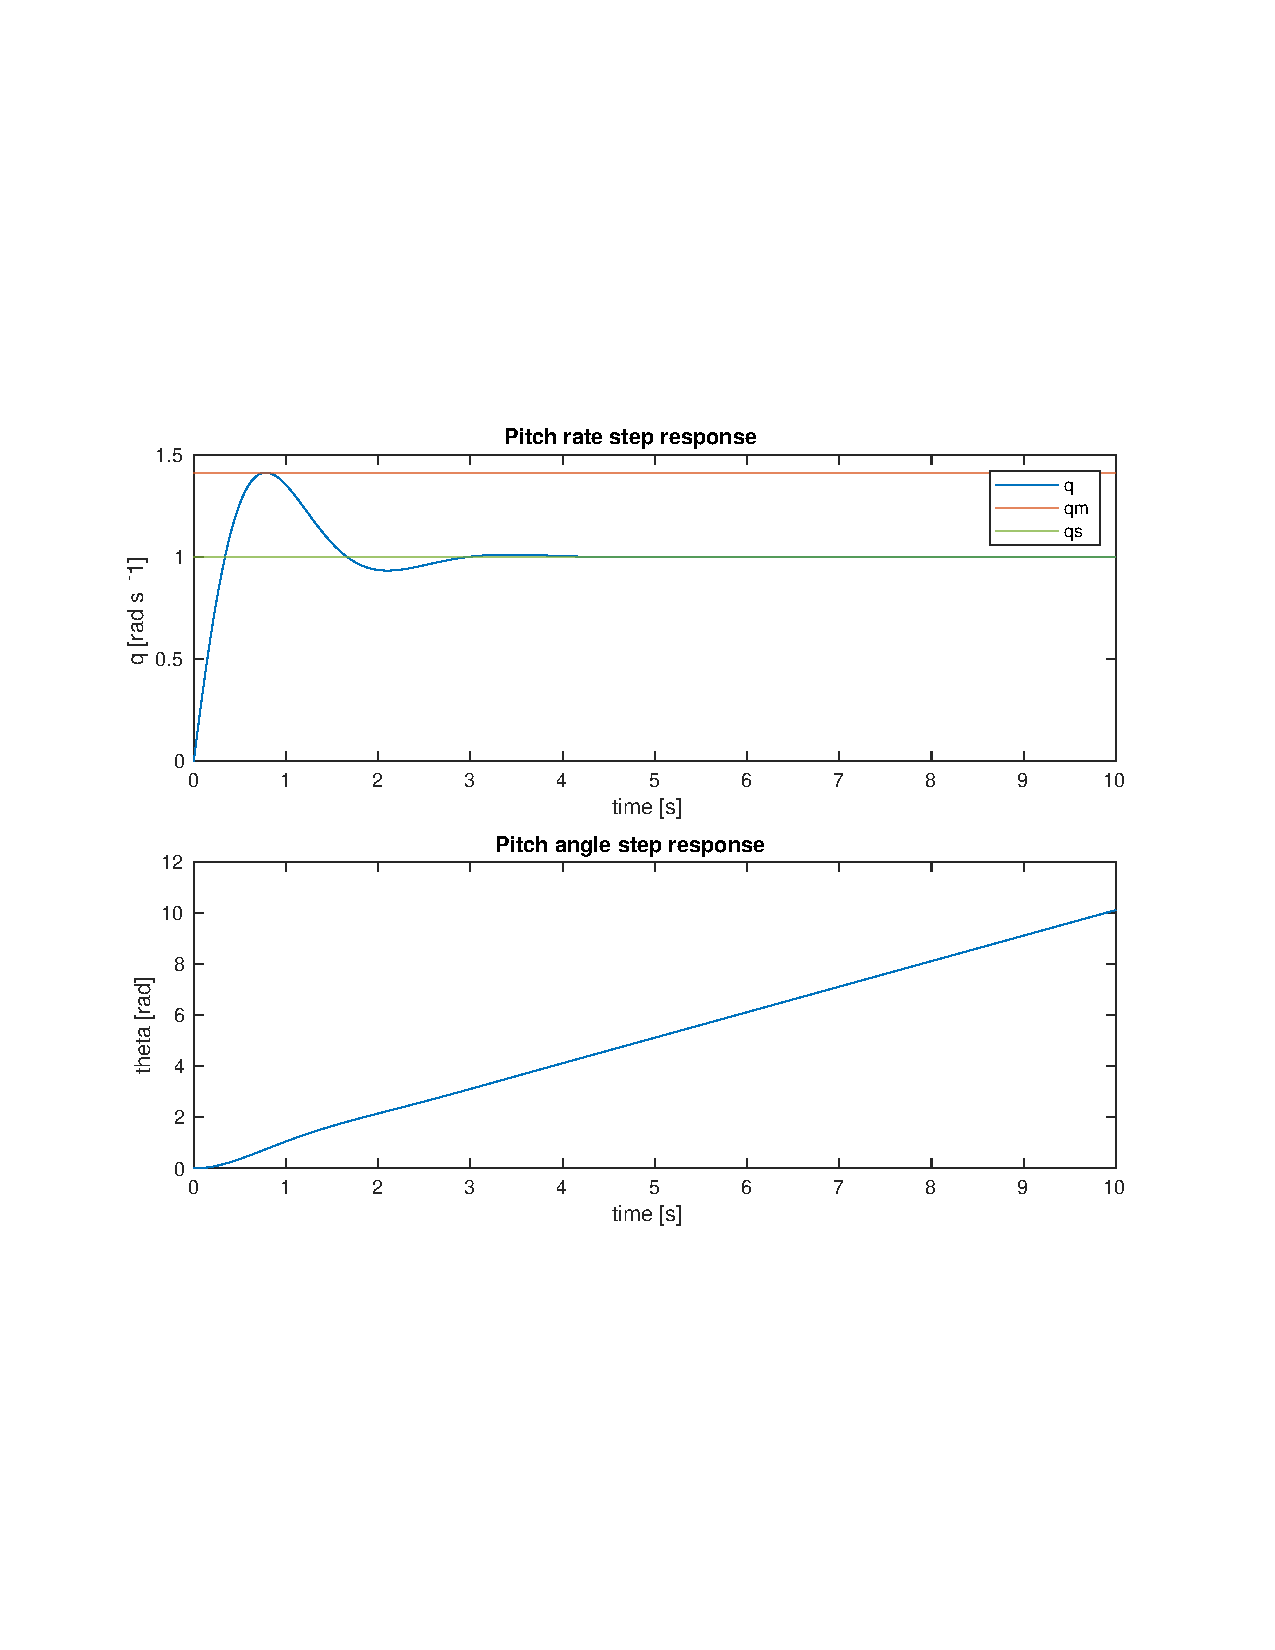
\includegraphics[width=0.8\textwidth]{figures/pc_pitch_resp.pdf}    
    \caption{Pitch rate and pitch angle step response of the controlled system.}
    \label{fig:pc_pitch_resp}
\end{figure}



Figure~\ref{fig:pc_cap} shows the satisfactory range of values to meet the Gibson dropback criterion. As it can be seen the controlled system satisfies the criteria.
\begin{align}
    \label{eq:gibvals}
    \frac{DB}{q_s} &= T_{\theta_2} - \frac{2\zeta_{sp}}{\omega_{n_{sp}}} \approx 0.1099 \\
    \frac{q_m}{q_s} &= \frac{1.4126}{1} = 1.4126
\end{align}

\begin{figure}[ht]
    \centering
    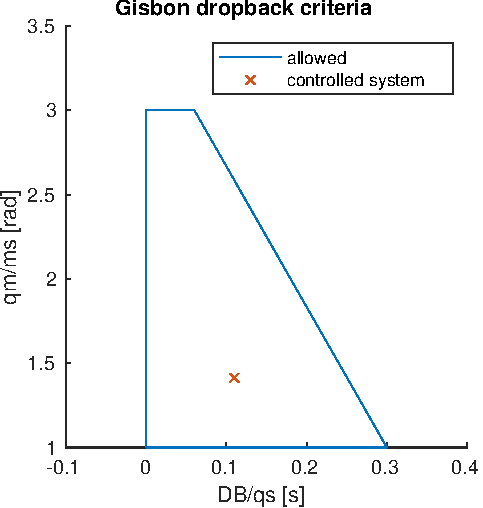
\includegraphics[width=0.4\textwidth]{figures/pc_gib.pdf}    
    \caption{Pitch rate and pitch angle step response of the controlled system.}
    \label{fig:pc_gib}
\end{figure}



\clearpage
